\section{Building Vision Models}
\begin{frame}{}
    \LARGE Computer Vision: \textbf{How Can We Build Vision Models?}
\end{frame}

\begin{frame}{How can we build vision models?}
\begin{itemize}
    \item So far, we’ve worked with tabular data, where each sample consists of structured features. We processed this data using Fully Connected Neural Networks.
\end{itemize}
\begin{figure}
\centering
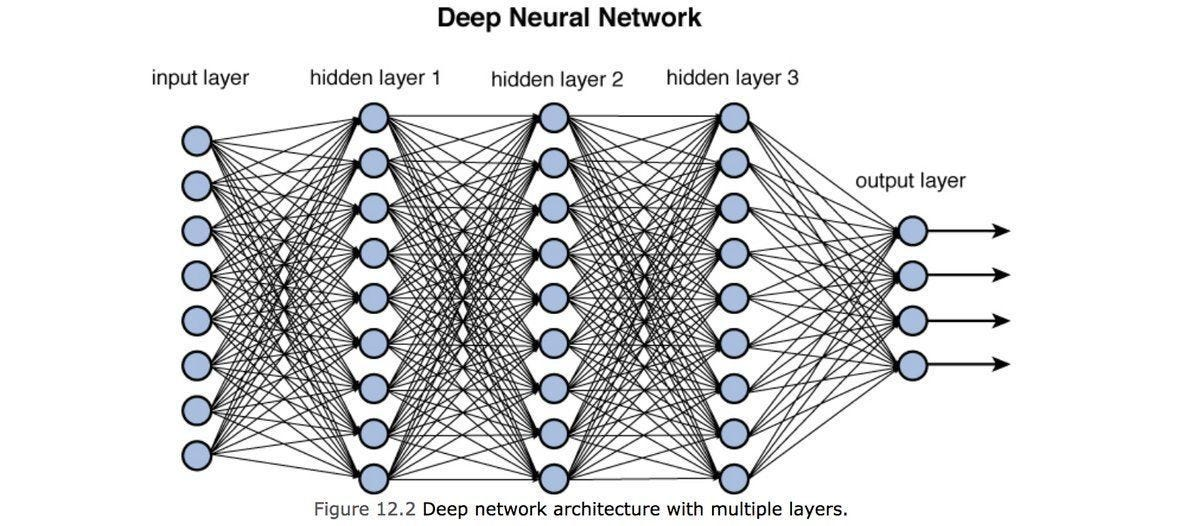
\includegraphics[width=1.0\textwidth,height=1.0\textheight,keepaspectratio]{images/cnn/nn.jpg}
\end{figure}
\begin{itemize}
    \item But can we apply the same approach to images?
\end{itemize}
\end{frame}

\begin{frame}{How can we build vision models?}
\begin{itemize}
    \item Let's try.
\end{itemize}
\end{frame}

\begin{frame}{How can we build vision models?}
\begin{itemize}
    \item Let's consider each pixel as a feature.
\end{itemize}

\begin{figure}
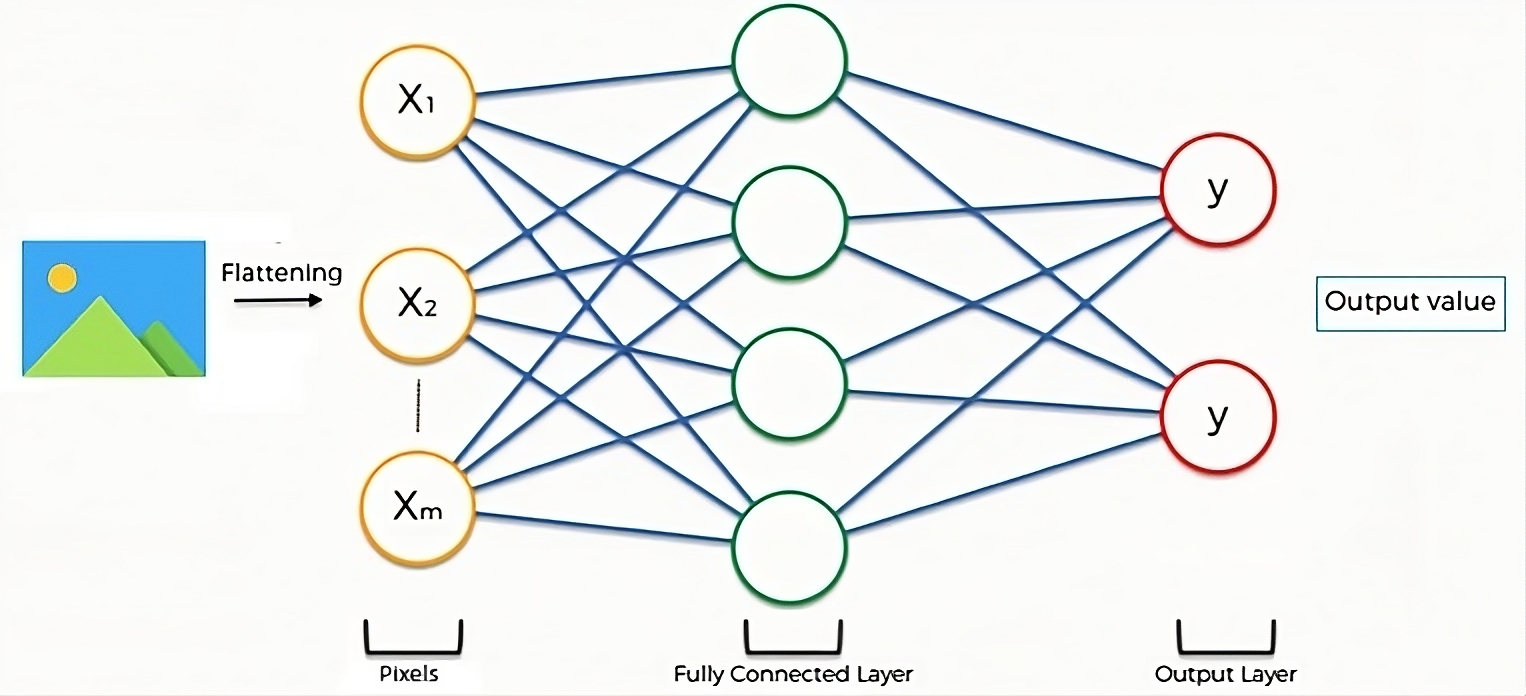
\includegraphics[width=1.0\textwidth,height=1.0\textheight,keepaspectratio]{images/cv-intro/images_nn.png}
\end{figure}
\begin{itemize}
    \item This should work! But...
\end{itemize}
\end{frame}
